% GNUPLOT: LaTeX picture with Postscript
\begingroup
  \makeatletter
  \providecommand\color[2][]{%
    \GenericError{(gnuplot) \space\space\space\@spaces}{%
      Package color not loaded in conjunction with
      terminal option `colourtext'%
    }{See the gnuplot documentation for explanation.%
    }{Either use 'blacktext' in gnuplot or load the package
      color.sty in LaTeX.}%
    \renewcommand\color[2][]{}%
  }%
  \providecommand\includegraphics[2][]{%
    \GenericError{(gnuplot) \space\space\space\@spaces}{%
      Package graphicx or graphics not loaded%
    }{See the gnuplot documentation for explanation.%
    }{The gnuplot epslatex terminal needs graphicx.sty or graphics.sty.}%
    \renewcommand\includegraphics[2][]{}%
  }%
  \providecommand\rotatebox[2]{#2}%
  \@ifundefined{ifGPcolor}{%
    \newif\ifGPcolor
    \GPcolortrue
  }{}%
  \@ifundefined{ifGPblacktext}{%
    \newif\ifGPblacktext
    \GPblacktexttrue
  }{}%
  % define a \g@addto@macro without @ in the name:
  \let\gplgaddtomacro\g@addto@macro
  % define empty templates for all commands taking text:
  \gdef\gplbacktext{}%
  \gdef\gplfronttext{}%
  \makeatother
  \ifGPblacktext
    % no textcolor at all
    \def\colorrgb#1{}%
    \def\colorgray#1{}%
  \else
    % gray or color?
    \ifGPcolor
      \def\colorrgb#1{\color[rgb]{#1}}%
      \def\colorgray#1{\color[gray]{#1}}%
      \expandafter\def\csname LTw\endcsname{\color{white}}%
      \expandafter\def\csname LTb\endcsname{\color{black}}%
      \expandafter\def\csname LTa\endcsname{\color{black}}%
      \expandafter\def\csname LT0\endcsname{\color[rgb]{1,0,0}}%
      \expandafter\def\csname LT1\endcsname{\color[rgb]{0,1,0}}%
      \expandafter\def\csname LT2\endcsname{\color[rgb]{0,0,1}}%
      \expandafter\def\csname LT3\endcsname{\color[rgb]{1,0,1}}%
      \expandafter\def\csname LT4\endcsname{\color[rgb]{0,1,1}}%
      \expandafter\def\csname LT5\endcsname{\color[rgb]{1,1,0}}%
      \expandafter\def\csname LT6\endcsname{\color[rgb]{0,0,0}}%
      \expandafter\def\csname LT7\endcsname{\color[rgb]{1,0.3,0}}%
      \expandafter\def\csname LT8\endcsname{\color[rgb]{0.5,0.5,0.5}}%
    \else
      % gray
      \def\colorrgb#1{\color{black}}%
      \def\colorgray#1{\color[gray]{#1}}%
      \expandafter\def\csname LTw\endcsname{\color{white}}%
      \expandafter\def\csname LTb\endcsname{\color{black}}%
      \expandafter\def\csname LTa\endcsname{\color{black}}%
      \expandafter\def\csname LT0\endcsname{\color{black}}%
      \expandafter\def\csname LT1\endcsname{\color{black}}%
      \expandafter\def\csname LT2\endcsname{\color{black}}%
      \expandafter\def\csname LT3\endcsname{\color{black}}%
      \expandafter\def\csname LT4\endcsname{\color{black}}%
      \expandafter\def\csname LT5\endcsname{\color{black}}%
      \expandafter\def\csname LT6\endcsname{\color{black}}%
      \expandafter\def\csname LT7\endcsname{\color{black}}%
      \expandafter\def\csname LT8\endcsname{\color{black}}%
    \fi
  \fi
  \setlength{\unitlength}{0.0500bp}%
  \begin{picture}(8206.00,12240.00)%
    \gplgaddtomacro\gplbacktext{%
      \csname LTb\endcsname%
      \put(688,8567){\makebox(0,0)[r]{\strut{}0}}%
      \csname LTb\endcsname%
      \put(688,9077){\makebox(0,0)[r]{\strut{}100}}%
      \csname LTb\endcsname%
      \put(688,9587){\makebox(0,0)[r]{\strut{}200}}%
      \csname LTb\endcsname%
      \put(688,10097){\makebox(0,0)[r]{\strut{}300}}%
      \csname LTb\endcsname%
      \put(688,10607){\makebox(0,0)[r]{\strut{}400}}%
      \csname LTb\endcsname%
      \put(688,11117){\makebox(0,0)[r]{\strut{}500}}%
      \csname LTb\endcsname%
      \put(688,11627){\makebox(0,0)[r]{\strut{}600}}%
      \csname LTb\endcsname%
      \put(820,8347){\makebox(0,0){\strut{} 0}}%
      \csname LTb\endcsname%
      \put(1538,8347){\makebox(0,0){\strut{} 5}}%
      \csname LTb\endcsname%
      \put(2256,8347){\makebox(0,0){\strut{} 10}}%
      \csname LTb\endcsname%
      \put(2974,8347){\makebox(0,0){\strut{} 15}}%
      \csname LTb\endcsname%
      \put(3692,8347){\makebox(0,0){\strut{} 20}}%
      \put(50,10097){\rotatebox{-270}{\makebox(0,0){\strut{}Counts}}}%
      \put(2256,8061){\makebox(0,0){\strut{}}}%
      \put(3347,11382){\makebox(0,0)[l]{\strut{}Pb}}%
    }%
    \gplgaddtomacro\gplfronttext{%
    }%
    \gplgaddtomacro\gplbacktext{%
      \csname LTb\endcsname%
      \put(4381,8567){\makebox(0,0)[r]{\strut{}0}}%
      \csname LTb\endcsname%
      \put(4381,8873){\makebox(0,0)[r]{\strut{}1000}}%
      \csname LTb\endcsname%
      \put(4381,9179){\makebox(0,0)[r]{\strut{}2000}}%
      \csname LTb\endcsname%
      \put(4381,9485){\makebox(0,0)[r]{\strut{}3000}}%
      \csname LTb\endcsname%
      \put(4381,9791){\makebox(0,0)[r]{\strut{}4000}}%
      \csname LTb\endcsname%
      \put(4381,10097){\makebox(0,0)[r]{\strut{}5000}}%
      \csname LTb\endcsname%
      \put(4381,10403){\makebox(0,0)[r]{\strut{}6000}}%
      \csname LTb\endcsname%
      \put(4381,10709){\makebox(0,0)[r]{\strut{}7000}}%
      \csname LTb\endcsname%
      \put(4381,11015){\makebox(0,0)[r]{\strut{}8000}}%
      \csname LTb\endcsname%
      \put(4381,11321){\makebox(0,0)[r]{\strut{}9000}}%
      \csname LTb\endcsname%
      \put(4381,11627){\makebox(0,0)[r]{\strut{}10000}}%
      \csname LTb\endcsname%
      \put(4513,8347){\makebox(0,0){\strut{} 0}}%
      \csname LTb\endcsname%
      \put(5470,8347){\makebox(0,0){\strut{} 5}}%
      \csname LTb\endcsname%
      \put(6427,8347){\makebox(0,0){\strut{} 10}}%
      \csname LTb\endcsname%
      \put(7384,8347){\makebox(0,0){\strut{} 15}}%
      \put(5948,8061){\makebox(0,0){\strut{}}}%
      \put(7039,11382){\makebox(0,0)[l]{\strut{}Fe}}%
    }%
    \gplgaddtomacro\gplfronttext{%
    }%
    \gplgaddtomacro\gplbacktext{%
      \csname LTb\endcsname%
      \put(688,4896){\makebox(0,0)[r]{\strut{}0}}%
      \csname LTb\endcsname%
      \put(688,5236){\makebox(0,0)[r]{\strut{}50}}%
      \csname LTb\endcsname%
      \put(688,5576){\makebox(0,0)[r]{\strut{}100}}%
      \csname LTb\endcsname%
      \put(688,5916){\makebox(0,0)[r]{\strut{}150}}%
      \csname LTb\endcsname%
      \put(688,6256){\makebox(0,0)[r]{\strut{}200}}%
      \csname LTb\endcsname%
      \put(688,6595){\makebox(0,0)[r]{\strut{}250}}%
      \csname LTb\endcsname%
      \put(688,6935){\makebox(0,0)[r]{\strut{}300}}%
      \csname LTb\endcsname%
      \put(688,7275){\makebox(0,0)[r]{\strut{}350}}%
      \csname LTb\endcsname%
      \put(688,7615){\makebox(0,0)[r]{\strut{}400}}%
      \csname LTb\endcsname%
      \put(688,7955){\makebox(0,0)[r]{\strut{}450}}%
      \csname LTb\endcsname%
      \put(820,4676){\makebox(0,0){\strut{} 0}}%
      \csname LTb\endcsname%
      \put(1299,4676){\makebox(0,0){\strut{} 5}}%
      \csname LTb\endcsname%
      \put(1777,4676){\makebox(0,0){\strut{} 10}}%
      \csname LTb\endcsname%
      \put(2256,4676){\makebox(0,0){\strut{} 15}}%
      \csname LTb\endcsname%
      \put(2735,4676){\makebox(0,0){\strut{} 20}}%
      \csname LTb\endcsname%
      \put(3213,4676){\makebox(0,0){\strut{} 25}}%
      \csname LTb\endcsname%
      \put(3692,4676){\makebox(0,0){\strut{} 30}}%
      \put(50,6425){\rotatebox{-270}{\makebox(0,0){\strut{}Counts}}}%
      \put(2256,4390){\makebox(0,0){\strut{}}}%
      \put(3347,7710){\makebox(0,0)[l]{\strut{}Au}}%
    }%
    \gplgaddtomacro\gplfronttext{%
    }%
    \gplgaddtomacro\gplbacktext{%
      \csname LTb\endcsname%
      \put(4381,4896){\makebox(0,0)[r]{\strut{}0}}%
      \csname LTb\endcsname%
      \put(4381,5236){\makebox(0,0)[r]{\strut{}20}}%
      \csname LTb\endcsname%
      \put(4381,5576){\makebox(0,0)[r]{\strut{}40}}%
      \csname LTb\endcsname%
      \put(4381,5916){\makebox(0,0)[r]{\strut{}60}}%
      \csname LTb\endcsname%
      \put(4381,6256){\makebox(0,0)[r]{\strut{}80}}%
      \csname LTb\endcsname%
      \put(4381,6595){\makebox(0,0)[r]{\strut{}100}}%
      \csname LTb\endcsname%
      \put(4381,6935){\makebox(0,0)[r]{\strut{}120}}%
      \csname LTb\endcsname%
      \put(4381,7275){\makebox(0,0)[r]{\strut{}140}}%
      \csname LTb\endcsname%
      \put(4381,7615){\makebox(0,0)[r]{\strut{}160}}%
      \csname LTb\endcsname%
      \put(4381,7955){\makebox(0,0)[r]{\strut{}180}}%
      \csname LTb\endcsname%
      \put(4513,4676){\makebox(0,0){\strut{} 0}}%
      \csname LTb\endcsname%
      \put(4992,4676){\makebox(0,0){\strut{} 5}}%
      \csname LTb\endcsname%
      \put(5470,4676){\makebox(0,0){\strut{} 10}}%
      \csname LTb\endcsname%
      \put(5949,4676){\makebox(0,0){\strut{} 15}}%
      \csname LTb\endcsname%
      \put(6427,4676){\makebox(0,0){\strut{} 20}}%
      \csname LTb\endcsname%
      \put(6906,4676){\makebox(0,0){\strut{} 25}}%
      \csname LTb\endcsname%
      \put(7384,4676){\makebox(0,0){\strut{} 30}}%
      \put(5948,4390){\makebox(0,0){\strut{}}}%
      \put(7039,7710){\makebox(0,0)[l]{\strut{}In}}%
    }%
    \gplgaddtomacro\gplfronttext{%
    }%
    \gplgaddtomacro\gplbacktext{%
      \csname LTb\endcsname%
      \put(688,1224){\makebox(0,0)[r]{\strut{}0}}%
      \csname LTb\endcsname%
      \put(688,1606){\makebox(0,0)[r]{\strut{}500}}%
      \csname LTb\endcsname%
      \put(688,1989){\makebox(0,0)[r]{\strut{}1000}}%
      \csname LTb\endcsname%
      \put(688,2371){\makebox(0,0)[r]{\strut{}1500}}%
      \csname LTb\endcsname%
      \put(688,2754){\makebox(0,0)[r]{\strut{}2000}}%
      \csname LTb\endcsname%
      \put(688,3136){\makebox(0,0)[r]{\strut{}2500}}%
      \csname LTb\endcsname%
      \put(688,3518){\makebox(0,0)[r]{\strut{}3000}}%
      \csname LTb\endcsname%
      \put(688,3901){\makebox(0,0)[r]{\strut{}3500}}%
      \csname LTb\endcsname%
      \put(688,4283){\makebox(0,0)[r]{\strut{}4000}}%
      \csname LTb\endcsname%
      \put(820,1004){\makebox(0,0){\strut{} 0}}%
      \csname LTb\endcsname%
      \put(1777,1004){\makebox(0,0){\strut{} 5}}%
      \csname LTb\endcsname%
      \put(2735,1004){\makebox(0,0){\strut{} 10}}%
      \csname LTb\endcsname%
      \put(3692,1004){\makebox(0,0){\strut{} 15}}%
      \put(-82,2753){\rotatebox{-270}{\makebox(0,0){\strut{}Counts}}}%
      \put(2256,674){\makebox(0,0){\strut{}Energie $E / \si{\kilo\electronvolt}$}}%
      \put(3347,4038){\makebox(0,0)[l]{\strut{}Cu}}%
    }%
    \gplgaddtomacro\gplfronttext{%
    }%
    \gplgaddtomacro\gplbacktext{%
      \csname LTb\endcsname%
      \put(4381,1224){\makebox(0,0)[r]{\strut{}0}}%
      \csname LTb\endcsname%
      \put(4381,1734){\makebox(0,0)[r]{\strut{}1000}}%
      \csname LTb\endcsname%
      \put(4381,2244){\makebox(0,0)[r]{\strut{}2000}}%
      \csname LTb\endcsname%
      \put(4381,2754){\makebox(0,0)[r]{\strut{}3000}}%
      \csname LTb\endcsname%
      \put(4381,3263){\makebox(0,0)[r]{\strut{}4000}}%
      \csname LTb\endcsname%
      \put(4381,3773){\makebox(0,0)[r]{\strut{}5000}}%
      \csname LTb\endcsname%
      \put(4381,4283){\makebox(0,0)[r]{\strut{}6000}}%
      \csname LTb\endcsname%
      \put(4513,1004){\makebox(0,0){\strut{} 0}}%
      \csname LTb\endcsname%
      \put(5470,1004){\makebox(0,0){\strut{} 5}}%
      \csname LTb\endcsname%
      \put(6427,1004){\makebox(0,0){\strut{} 10}}%
      \csname LTb\endcsname%
      \put(7384,1004){\makebox(0,0){\strut{} 15}}%
      \put(5948,674){\makebox(0,0){\strut{}Energie $E / \si{\kilo\electronvolt}$}}%
      \put(7039,4038){\makebox(0,0)[l]{\strut{}Ni}}%
    }%
    \gplgaddtomacro\gplfronttext{%
    }%
    \gplbacktext
    \put(0,0){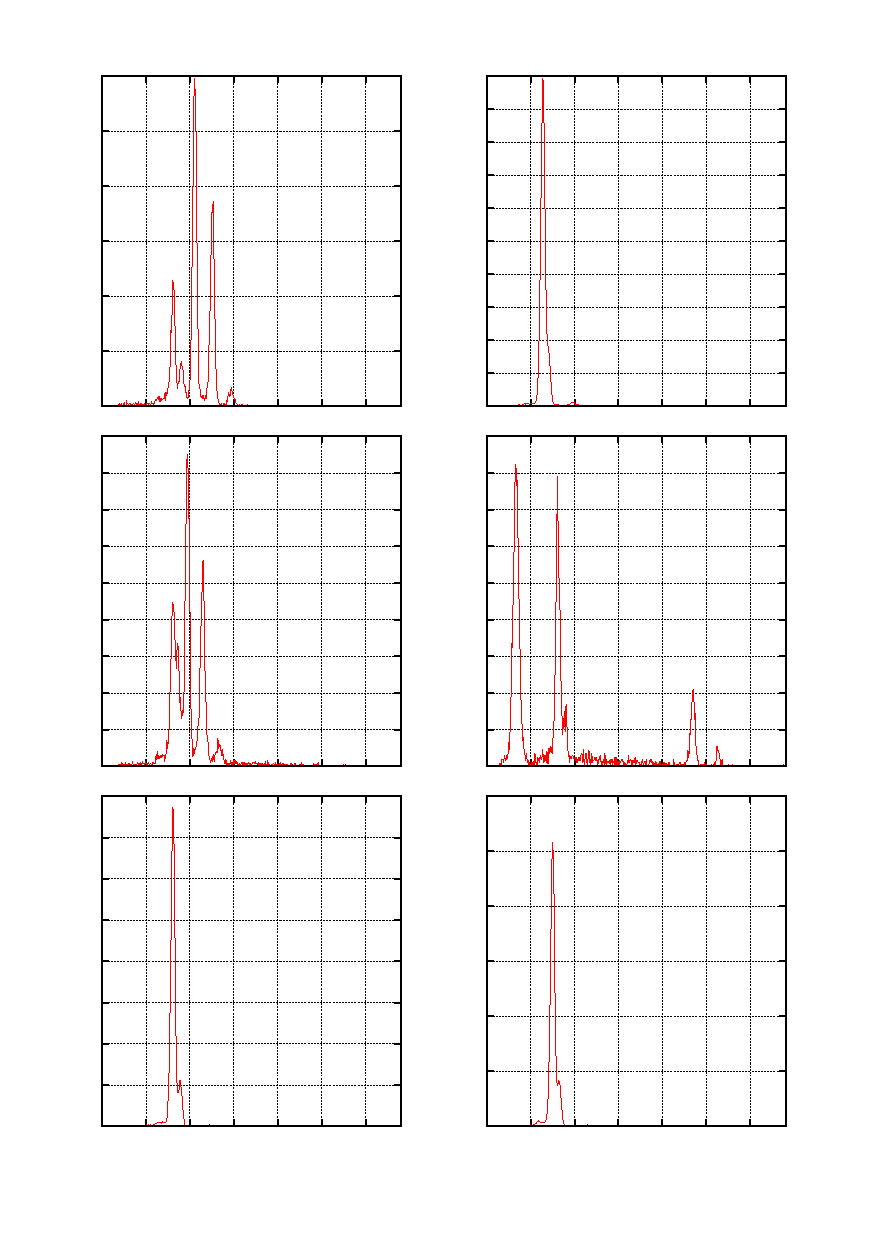
\includegraphics{./plots/referenzspektren1}}%
    \gplfronttext
  \end{picture}%
\endgroup
